\section{Introduction}
\emph{We are given an array that contains N numbers and would like to determine if there are two numbers whose sum equals a given number K.\\
For example we may be given the sequence 4,1,5,2,6,3 and are asked to find a pair of numbers with a sum of 10. In this example 4 and 6 is a valid result.\\
To solve the portfolio do the following:}
\begin{itemize}
\item \emph{Implement an O(\(N^{2}\)) algorithm for solving the problem.}
\item \emph{Implement an O(N Log(N)) algorithm for solving the problem. (Hint: Consider sorting the list.)}
\item \emph{Perform experiments with different values of N (generate the associated random lists yourselves)
and plot the time as function of N, to verify the time complexity.}
\end{itemize}
\emph{You may use a build in sorting algorithm and assume that it sorts in N Log(N).}

\section{Use of algorithms}
\todo[inline]{short introduction}
\subsection{O(\(N^{2}\))}
\todo[inline]{Description af the algorithm}
\todo[inline]{Pseudocode}
\subsection{O(N Log(N)}
\todo[inline]{Description af the algorithm}
\todo[inline]{Pseudocode}

\section{Verify the time complexity}

\subsection{O(\(N^{2}\))}
\todo[inline]{Description of the plot}
\begin{figure}[th!]
\centering
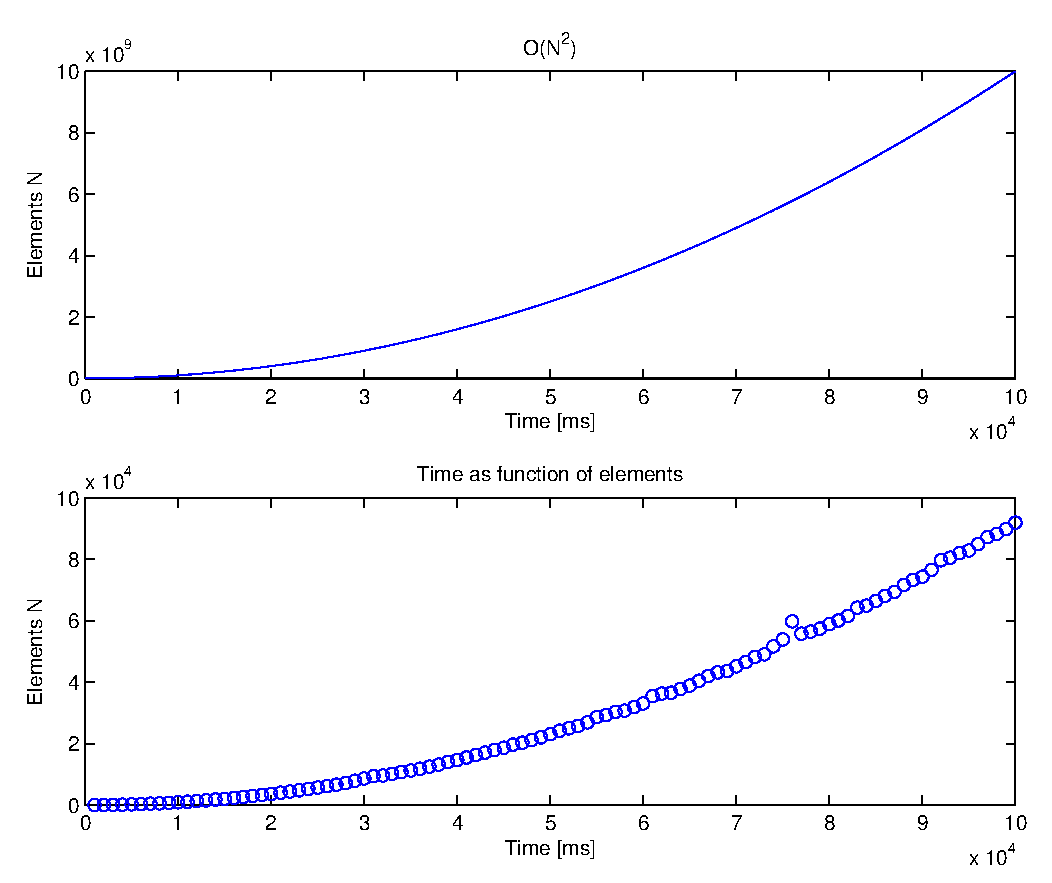
\includegraphics[width=1\textwidth]{./graphics/test1.eps}
\caption[tekst i indholdsfortegnelsen]{figurtekst}
\label{fig:}
\end{figure}

\subsection{O(N Log(N)}
\todo[inline]{Description of the plot}
\begin{figure}[th!]
\centering
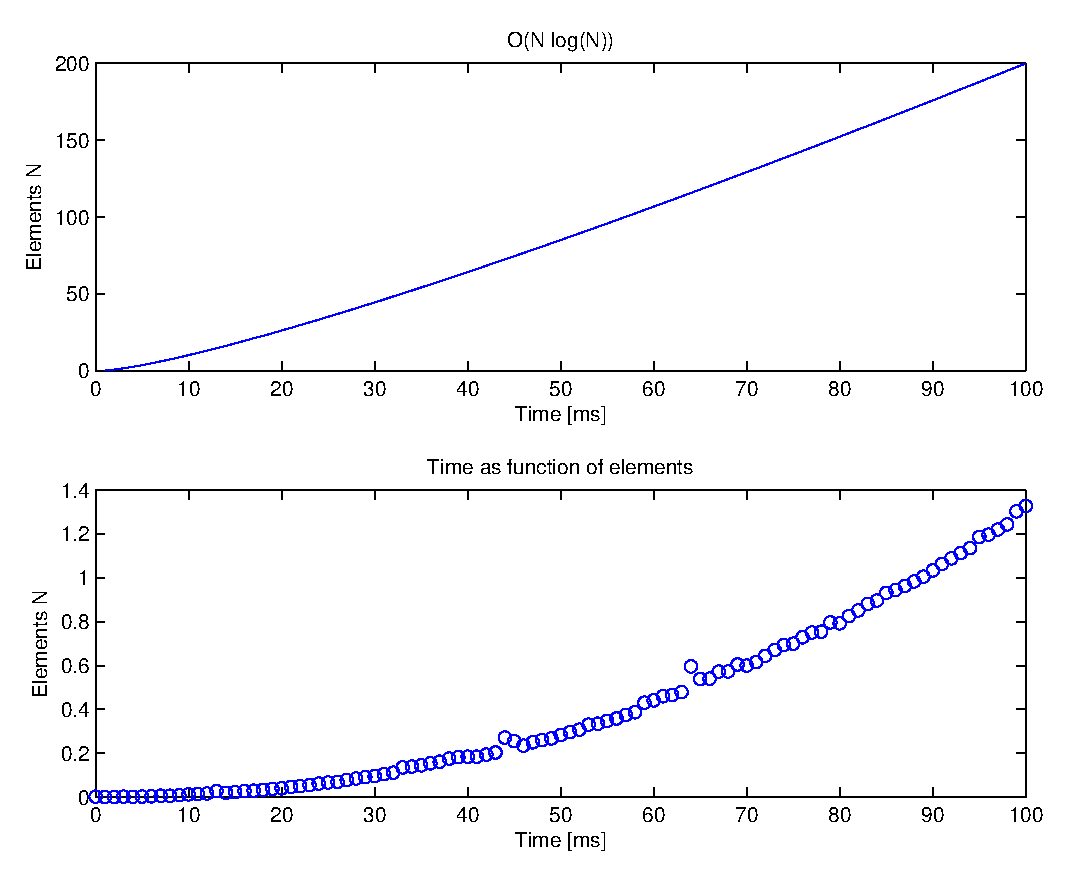
\includegraphics[width=1\textwidth]{./graphics/test2.eps}
\caption[tekst i indholdsfortegnelsen]{figurtekst}
\label{fig:}
\end{figure}